% !TeX TS-program = xelatex

\documentclass[10pt]{beamer}

\usetheme[progressbar=frametitle]{metropolis}
\usepackage{appendixnumberbeamer}
\usepackage{pgfplots}
\usepackage{xspace}

\newcommand{\themename}{\textbf{\textsc{metropolis}}\xspace}
%\setsansfont[BoldFont={Fira Sans}]{Fira Sans Light}
%\setmonofont{Fira Mono}
%\usepackage[sfdefault]{Fira Sans}

\title{}
\subtitle{}

\author{}

\date{EE/GW meeting, November 11, 2023}

\begin{document}
	
	\maketitle
	
	\begin{frame}{}
	
	\begin{itemize}
		\item Problem = overly narrow,biased posteriors 
	\end{itemize}

\end{frame}



\begin{frame}{}
	A match made in heaven: reduced precision + stochastic rounding \newline 
	
	   \centering
		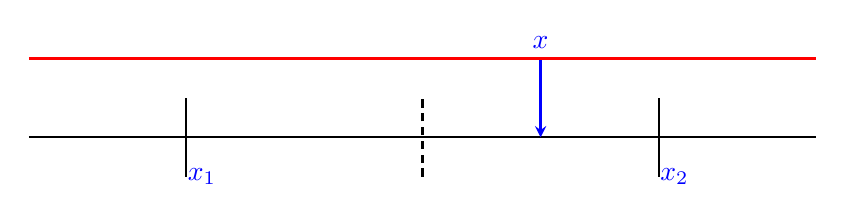
\begin{tikzpicture}
    \draw [-,>=stealth, color = black, thick] (-5, 0.0) -- (+5, 0.0); 
     \draw [densely dashed,>=stealth, color = black, thick] (0.0, -0.50) -- (0.0, +0.5); 
      \draw [-,>=stealth, color = black, thick] (-3, -0.50) -- (-3, +0.5); 
	\draw [-,>=stealth, color = black, thick] (+3, -0.50) -- (+3, +0.5); 
	\node[text=blue] at (3.2, -0.5) {$x_2$};
	\node[text=blue] at (-2.8, -0.5) {$x_1$};
	\node[text=blue] at (1.5, 1.2) {$x$};
	\draw [-stealth,color = blue, thick] (1.5, 1.01) -- (1.5, 0.0); 
		
	\draw [-,>=stealth, color = red, thick] (-5, 1.0) -- (+5, 1.0); 
		
	\end{tikzpicture}

\raggedright

\begin{itemize}
	\item Usual way: Round-to-nearest
	\item Alternatively: Round \alert{stochastically} 
\end{itemize}

Why bother? $\rightarrow \mathbb{E} \left(\mathcal{R}(x)\right) = x$

	
\end{frame}






\begin{frame}{}
\centering
\vspace{5mm}
%\includegraphics[width=0.75\textwidth,height=0.75\textwidth]{images/precip_ensemble_timeseries_decadal}

\raggedleft
\vspace{-1mm}
\tiny \url{arxiv.org/abs/2207.14598} \normalsize

\end{frame}





%	\begin{frame}{}
	%
	%Numerical weather and climate modelling 
	%
	%        \begin{itemize}
		%	        \item Reduced precision floats + stochastic rounding
		%	        \item Automatic Differentiation
		%        \end{itemize}
	%    
	%    \alert{Open call for collaboration!}
	%    
	%    
	%	\end{frame}



	
\end{document}